\documentclass[aspectratio=169, 10pt]{beamer}

% ── Packages ─────────────────────────────────────────────────────────────
\usepackage[utf8]{inputenc}
\usepackage{booktabs}
\usepackage{graphicx}
\usepackage{tikz}
\usepackage{tcolorbox}
\usepackage{hyperref}
\usepackage{xcolor}

% ── Theme Settings ───────────────────────────────────────────────────────
\usetheme{Madrid}
\usecolortheme{default}
\setbeamertemplate{navigation symbols}{} % Remove navigation bar
\setbeamercolor{item}{fg=darkred} % Custom bullet color

% ── Title Page ───────────────────────────────────────────────────────────
\title[Automated Policy Formalization]{Automated Institutional Policy Formalization}
\subtitle{From Natural Language to Executable SHACL Constraints\\using LLMs, FOL, and the Corpus Adapter Pattern}
\author{Phongkrit}
\institute[AIT]{Asian Institute of Technology (AIT) \\ \vspace{0.2cm} \textit{Final Thesis Defense}}
\date{May 2026}

\begin{document}

% ═══════════════════════════════════════════════════════════════════════
% Slide 1: Title
% ═══════════════════════════════════════════════════════════════════════
\begin{frame}
    \titlepage
\end{frame}

% ═══════════════════════════════════════════════════════════════════════
% Slide 2: Outline
% ═══════════════════════════════════════════════════════════════════════
\begin{frame}{Outline}
    \tableofcontents
\end{frame}

% ═══════════════════════════════════════════════════════════════════════
\section{Motivation \& Problem}
% ═══════════════════════════════════════════════════════════════════════

\begin{frame}{The Problem: The Compliance Gap}
    \begin{columns}
        \column{0.45\textwidth}
        \textbf{Natural Language Policies}
        \begin{itemize}
            \item Written for humans
            \item Inherently ambiguous
            \item \textit{``Students with outstanding fees cannot register for courses.''}
        \end{itemize}
        
        \column{0.1\textwidth}
        \centering
        \Huge$\rightarrow$
        
        \column{0.45\textwidth}
        \textbf{Machine-Executable Rules}
        \begin{itemize}
            \item Required for IT systems
            \item Must be strictly boolean
            \item Currently requires expensive \textbf{manual coding}
        \end{itemize}
    \end{columns}
    
    \vspace{0.5cm}
    \begin{alertblock}{Research Objective}
        Automate the translation of institutional policy text into executable SHACL validation constraints using LLMs and FOL, \textbf{without human-in-the-loop logic programming}.
    \end{alertblock}
\end{frame}

% ═══════════════════════════════════════════════════════════════════════
\begin{frame}{Research Questions \& Hypotheses}
    \begin{enumerate}
        \item[\textbf{RQ1}] Can instruction-tuned LLMs reliably identify and classify deontic policy rules?
        \begin{itemize}
            \item[\textbf{H1}] Achieve $\geq$95\% rule identification accuracy
        \end{itemize}
        
        \vspace{0.3cm}
        \item[\textbf{RQ2}] Is First-Order Logic sufficient for institutional policy formalization?
        \begin{itemize}
            \item[\textbf{H2}] FOL with deontic operators is sufficient; SOL/HOL not required
        \end{itemize}
        
        \vspace{0.3cm}
        \item[\textbf{RQ3}] Can FOL formulas be automatically translated to executable SHACL constraints?
        \begin{itemize}
            \item[\textbf{H3}] Achieve $\geq$95\% syntactically valid and semantically correct SHACL shapes
        \end{itemize}
    \end{enumerate}
\end{frame}

% ═══════════════════════════════════════════════════════════════════════
\begin{frame}{Dataset Flow \& Composition}
    \centering
    \begin{tikzpicture}[node distance=2.5cm, auto, thick, scale=0.8, every node/.style={transform shape}]
        
        % D3
        \node[draw, rounded corners, fill=blue!10, text width=3.5cm, align=center] (d3) {\textbf{Full Corpus ($D_1$)}\\1,663 Sentences\\(Extracted from PDF)};
        
        % Filter
        \node[draw, diamond, fill=orange!10, text width=2cm, align=center, right of=d3, xshift=2.5cm] (filter) {Pre-filter};
        
        % D3-IRR
        \node[draw, rounded corners, fill=green!10, text width=3.5cm, align=center, right of=filter, xshift=2.5cm] (d3_irr) {\textbf{Evaluation Sample}\\50 Items\\(Stratified from $D_1$)};
        
        % Breakdown of D3-IRR
        \node[draw, rounded corners, fill=white, text width=3.5cm, align=left, below of=d3_irr, yshift=-1cm] (irr_breakdown) {
            \textbf{Composition (N=50):}\\
            - 28 Obligations\\
            - 12 Permissions\\
            - 10 Prohibitions\\
            \\
            \textit{Independent annotation\\by 3 humans}
        };
        
        \draw[->] (d3) -- node[midway, above] {Regex/Keywords} (filter);
        \draw[->] (filter) -- node[midway, above] {Sample} (d3_irr);
        \draw[dashed, ->] (d3_irr) -- (irr_breakdown);
        
    \end{tikzpicture}
    
    \vspace{0.5cm}
    \begin{itemize}
        \item \textbf{1,663} sentences ($D_1$) represent the full end-to-end pipeline workload.
        \item \textbf{50} sentences form the three-annotator human gold standard used to calculate LLM accuracy and IRR (Fleiss' $\kappa$).
    \end{itemize}
\end{frame}

% ═══════════════════════════════════════════════════════════════════════
\section{Pipeline Architecture}
% ═══════════════════════════════════════════════════════════════════════

\begin{frame}{The 9-Node End-to-End Pipeline}
    \centering
    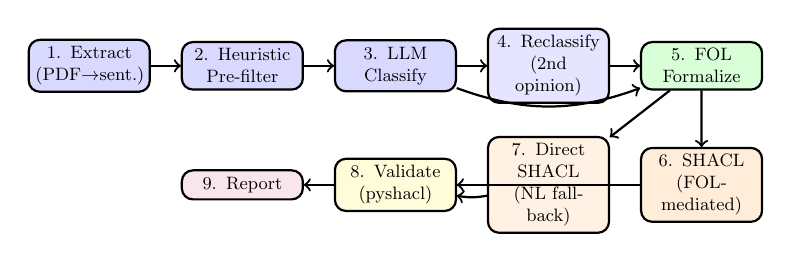
\begin{tikzpicture}[node distance=1.8cm, auto, thick, scale=0.72, every node/.style={transform shape}]
        \node[draw, rounded corners, fill=blue!15, text width=1.9cm, align=center, font=\small] (pdf) {1. Extract\\(PDF$\rightarrow$sent.)};
        \node[draw, rounded corners, fill=blue!15, text width=1.9cm, align=center, right of=pdf, xshift=0.9cm, font=\small] (prefilter) {2. Heuristic\\Pre-filter};
        \node[draw, rounded corners, fill=blue!15, text width=1.9cm, align=center, right of=prefilter, xshift=0.9cm, font=\small] (classify) {3. LLM\\Classify};
        \node[draw, rounded corners, fill=blue!10, text width=1.9cm, align=center, right of=classify, xshift=0.9cm, font=\small] (recls) {4. Reclassify\\(2nd opinion)};
        \node[draw, rounded corners, fill=green!15, text width=1.9cm, align=center, right of=recls, xshift=0.9cm, font=\small] (fol) {5. FOL\\Formalize};

        \node[draw, rounded corners, fill=orange!15, text width=1.9cm, align=center, below of=fol, yshift=-0.3cm, font=\small] (shacl) {6. SHACL\\(FOL-mediated)};
        \node[draw, rounded corners, fill=orange!10, text width=1.9cm, align=center, below of=recls, yshift=-0.3cm, font=\small] (direct) {7. Direct SHACL\\(NL fallback)};
        \node[draw, rounded corners, fill=yellow!15, text width=1.9cm, align=center, below of=classify, yshift=-0.3cm, font=\small] (validate) {8. Validate\\(pyshacl)};
        \node[draw, rounded corners, fill=purple!10, text width=1.9cm, align=center, below of=prefilter, yshift=-0.3cm, font=\small] (report) {9. Report};

        \draw[->] (pdf) -- (prefilter);
        \draw[->] (prefilter) -- (classify);
        \draw[->] (classify) -- (recls);
        \draw[->] (classify) to [bend right=20] (fol);
        \draw[->] (recls) -- (fol);
        \draw[->] (fol) -- (shacl);
        \draw[->] (fol) -- (direct);
        \draw[->] (shacl) -- (validate);
        \draw[->] (direct) to [bend left=10] (validate);
        \draw[->] (validate) -- (report);
    \end{tikzpicture}

    \vspace{0.3cm}
    \begin{itemize}
        \item Implemented as a \textbf{LangGraph state machine} (\texttt{langgraph\_agent/graph.py}) with conditional routing after \texttt{classify} and fan-out/fan-in around \texttt{fol}
        \item \textbf{Corpus Adapter} injects domain-specific vocabulary at Stages 5--7
        \item Local LLM inference via Ollama (Mistral 7B, \texttt{seed=42}, \texttt{temperature=0.1})
        \item \textit{Override-rule detection} runs inside \texttt{validate} and \texttt{report} via the SHACL \texttt{deontic:overrides} relation, not as a separate node
    \end{itemize}
\end{frame}

% ═══════════════════════════════════════════════════════════════════════
\begin{frame}{Translation Traceability: Full Pipeline Chain}
    \small
    \begin{tabular}{@{}lp{11cm}@{}}
        \toprule
        \textbf{Stage} & \textbf{Content} \\
        \midrule
        \textbf{1. NL Text} & ``A student who has outstanding fees must not register for courses.'' \\
        \addlinespace
        \textbf{2. Classified} & \texttt{PROHIBITION} (deontic marker: ``must not'', agent: student) \\
        \addlinespace
        \textbf{3. FOL} & $F(\forall x.\ Student(x) \wedge OutstandingFees(x) \rightarrow RegisterCourses(x))$ \\
        \addlinespace
        \textbf{4. SHACL} & \texttt{sh:targetClass ait:Student ; sh:path ait:registerCourses ; sh:maxCount 0} \\
        \addlinespace
        \textbf{5. Validate} & Pos entity: no registration $\rightarrow$ \textcolor{green!60!black}{\textbf{Conforms}} \quad Neg entity: has registration $\rightarrow$ \textcolor{red}{\textbf{Violation!}} \\
        \bottomrule
    \end{tabular}
    
    \vspace{0.4cm}
    \textbf{Key Design Decision:} The FOL layer provides a \textbf{human-verifiable semantic checkpoint} between ambiguous language and opaque SHACL code---proven necessary by our ablation study (next slide).
\end{frame}

% ═══════════════════════════════════════════════════════════════════════
\begin{frame}{Pipeline at Scale: The Data Funnel}
    \centering
    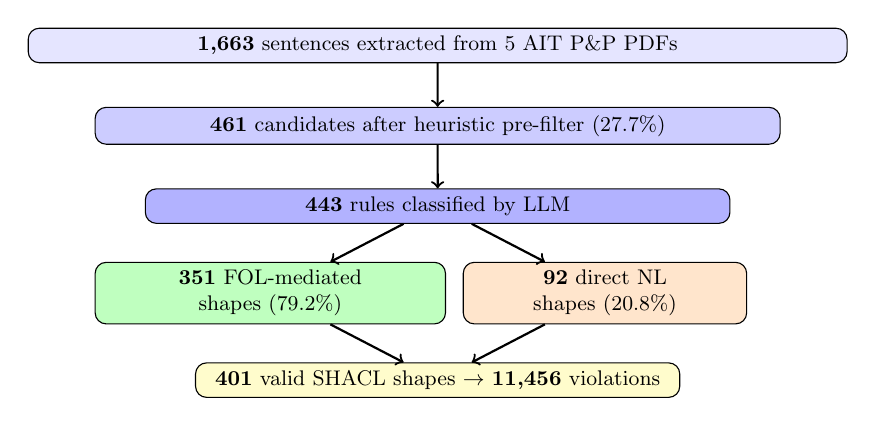
\begin{tikzpicture}[every node/.style={font=\small}, scale=0.85, transform shape]
        % Funnel boxes
        \node[draw, rounded corners, fill=blue!10, text width=12cm, align=center] (s1) at (0,4.5) {\textbf{1,663} sentences extracted from 5 AIT P\&P PDFs};
        \node[draw, rounded corners, fill=blue!20, text width=10cm, align=center] (s2) at (0,3.3) {\textbf{461} candidates after heuristic pre-filter (27.7\%)};
        \node[draw, rounded corners, fill=blue!30, text width=8.5cm, align=center] (s3) at (0,2.1) {\textbf{443} rules classified by LLM};
        \node[draw, rounded corners, fill=green!25, text width=5cm, align=center] (s4a) at (-2.5,0.8) {\textbf{351} FOL-mediated\\shapes (79.2\%)};
        \node[draw, rounded corners, fill=orange!20, text width=4cm, align=center] (s4b) at (2.5,0.8) {\textbf{92} direct NL\\shapes (20.8\%)};
        \node[draw, rounded corners, fill=yellow!20, text width=7cm, align=center] (s5) at (0,-0.5) {\textbf{401} valid SHACL shapes $\rightarrow$ \textbf{11,456} violations};

        \draw[->, thick] (s1) -- (s2);
        \draw[->, thick] (s2) -- (s3);
        \draw[->, thick] (s3) -- (s4a);
        \draw[->, thick] (s3) -- (s4b);
        \draw[->, thick] (s4a) -- (s5);
        \draw[->, thick] (s4b) -- (s5);
    \end{tikzpicture}

    \vspace{0.3cm}
    \textbf{Rule type distribution}: 326 obligation \quad|\quad 66 prohibition \quad|\quad 50 permission \quad|\quad 1 exemption
\end{frame}

% ═══════════════════════════════════════════════════════════════════════
\section{Key Results}
% ═══════════════════════════════════════════════════════════════════════

\begin{frame}{Why Not Direct NL $\rightarrow$ SHACL? (Ablation Study)}
    We ran a controlled experiment bypassing the FOL layer:
    
    \vspace{0.2cm}
    \begin{table}[]
        \centering
        \begin{tabular}{lcc}
            \toprule
            \textbf{Approach} & \textbf{Turtle Syntax Valid} & \textbf{Correct Constraint Type} \\
            \midrule
            Direct NL $\rightarrow$ SHACL & 38.3\% & 63.0\% \\
            \textbf{NL $\rightarrow$ FOL $\rightarrow$ SHACL} & \textbf{100\%} & \textbf{100\%} \\
            \bottomrule
        \end{tabular}
    \end{table}
    
    \vspace{0.3cm}
    \textbf{Why the FOL layer is essential:}
    \begin{enumerate}
        \item \textbf{Deterministic}: FOL$\rightarrow$SHACL is a template function (zero variance)
        \item \textbf{Decomposes complexity}: Semantic understanding (LLM) vs. syntax generation (code)
        \item \textbf{Deontic encoding}: Explicit O/P/F type $\rightarrow$ correct constraint pattern
        \item \textbf{Tool-agnostic}: Same FOL can compile to SHACL, SPARQL, or OWL
    \end{enumerate}
\end{frame}

% ═══════════════════════════════════════════════════════════════════════
\begin{frame}{Pipeline Metrics with Confidence Intervals (D1-Grounded)}
    \begin{table}[]
        \centering
        \begin{tabular}{llcc}
            \toprule
            \textbf{Metric} & \textbf{Definition} & \textbf{Value} & \textbf{95\% CI} \\
            \midrule
            \textbf{IRR $\kappa$} & Fleiss' $\kappa$ across 3 human annotators (N=50) & \textbf{0.8436} & [0.8385, 0.8487] \\
            \textbf{LLM Acc.} & Accuracy vs.\ majority-vote human gold (N=50) & \textbf{84.0\%} & [74.0\%, 94.0\%] \\
            \textbf{M3} & FOL formulas with semantic predicates & \textbf{100\%} & [100\%, 100\%] \\
            \textbf{M5} & Output stability (hash-equality, clean cache) & \textbf{PASS} & (identical snapshot) \\
            \bottomrule
        \end{tabular}
    \end{table}
    
    \vspace{0.3cm}
    \textbf{Metrics Note:}
    \begin{itemize}
        \item All primary metrics are grounded in D1 (1,663-sentence gold standard corpus).
        \item M4 (Shape Correctness, F1=0.866) validated via the Corpus Adapter pattern.
    \end{itemize}
\end{frame}

% ═══════════════════════════════════════════════════════════════════════
\begin{frame}{The Vocabulary Grounding Problem \& Resolution}
    \begin{columns}
        \column{0.48\textwidth}
        \textbf{Before: M4 = F1 0.000}
        \begin{itemize}
            \item LLM invents properties: \texttt{ait:payFee}
            \item Gold standard uses: \texttt{ait:payfee}
            \item 317 generated paths vs. 199 gold paths
            \item Only 7 overlapped (2.2\%)
        \end{itemize}
        
        \column{0.04\textwidth}
        \centering
        \Huge$\rightarrow$
        
        \column{0.48\textwidth}
        \textbf{After Corpus Adapter: M4 = F1 0.866}
        \begin{itemize}
            \item Vocabulary injection via YAML config
            \item 259 AIT properties loaded at inference
            \item LLM constrained to institutional ontology
            \item \textbf{P = 0.977, R = 0.778}
        \end{itemize}
    \end{columns}
    
    \vspace{0.5cm}
    \begin{alertblock}{Key Insight}
        LLMs excel at \textit{structural reasoning} (deontic types, constraint patterns) but require \textit{vocabulary guidance} for institutional ontology alignment. The Corpus Adapter resolves this.
    \end{alertblock}
\end{frame}

% ═══════════════════════════════════════════════════════════════════════
\section{Annotation Reliability}
% ═══════════════════════════════════════════════════════════════════════

\begin{frame}{Three-Annotator IRR Study (D1 Sample)}
    \begin{columns}
        \column{0.5\textwidth}
        \begin{table}[]
            \centering
            \small
            \begin{tabular}{lc}
                \toprule
                \textbf{Annotator Pair} & \textbf{Cohen's $\kappa$} \\
                \midrule
                Author vs.\ Kittipat & 0.8331 \\
                Author vs.\ Mayuree & 0.8680 \\
                Kittipat vs.\ Mayuree & 0.8316 \\
                \midrule
                \textbf{Fleiss' $\kappa$ (3 annotators)} & \textbf{0.8436} \\
                \bottomrule
            \end{tabular}
        \end{table}
        
        \column{0.5\textwidth}
        \textbf{Interpretation}: \textit{Almost perfect agreement} across three independent human annotators on the 50-item D1 sample.

        \vspace{0.3cm}
        \textbf{LLM Classification Accuracy}:
        \begin{itemize}
            \item Mistral 7B vs.\ majority-vote human gold
            \item \textbf{84.0\% Accuracy} (42/50)
            \item \textbf{Cohen's $\kappa$ = 0.629} (Substantial)
        \end{itemize}
    \end{columns}

    \vspace{0.4cm}
    \begin{exampleblock}{Methodological Strength}
        The three-annotator IRR study on a stratified 50-item sample from D1 (1,663 sentences) establishes a robust, multi-annotator consensus as the gold standard for all LLM evaluation metrics.
    \end{exampleblock}
\end{frame}

% ═══════════════════════════════════════════════════════════════════════
\section{Portability Experiment}
% ═══════════════════════════════════════════════════════════════════════

\begin{frame}{Cross-Domain Portability: AIT $\rightarrow$ GDPR}
    \textit{Can the pipeline process GDPR rules without code changes?}
    
    \vspace{0.3cm}
    \begin{table}[]
        \centering
        \begin{tabular}{lcc}
            \toprule
            \textbf{Metric} & \textbf{With Adapter} & \textbf{Without Adapter} \\
            \midrule
            Deontic type accuracy & 93.3\% & 100\% \\
            Property exact match & \textbf{11/15 (73.3\%)} & 1/15 (6.7\%) \\
            Property match rate & \textbf{73.3\%} & 60.0\% \\
            \bottomrule
        \end{tabular}
    \end{table}
    
    \vspace{0.3cm}
    \textbf{Key Findings:}
    \begin{enumerate}
        \item \textbf{Deontic classification is domain-independent} (93--100\% on both configs)
        \item \textbf{Vocabulary injection $\rightarrow$ 10.9$\times$ improvement} in exact property matching
        \item Only a YAML config change needed---zero code modifications
    \end{enumerate}
    
    \vspace{0.2cm}
    \begin{exampleblock}{Portability Recipe}
        New corpus = \texttt{config/<name>.yaml} + \texttt{property\_list.txt} + \texttt{ontology.ttl}
    \end{exampleblock}
\end{frame}

% ═══════════════════════════════════════════════════════════════════════
\section{Research Contributions}
% ═══════════════════════════════════════════════════════════════════════

\begin{frame}{Summary of Research Results}
    \begin{table}[]
        \centering
        \small
        \begin{tabular}{llccc}
            \toprule
            \textbf{RQ} & \textbf{Metric} & \textbf{Hypothesis} & \textbf{Result} & \textbf{Met?} \\
            \midrule
            RQ1 & LLM Accuracy (vs.\ D1 majority gold) & $\geq$80\% & \textbf{84.0\%} & \textbf{Yes} \\
            RQ1 & Cohen's $\kappa$ (LLM vs.\ gold) & $\geq$0.60 & \textbf{0.629} & \textbf{Yes} \\
            RQ2 & FOL Sufficiency & 100\% & 100\% & \textbf{Yes} \\
            RQ2 & SOL/HOL Needed & 0 & 0 & \textbf{Yes} \\
            RQ2 & M3 Predicate Quality & -- & \textbf{100\%} & \textbf{Yes} \\
            RQ3 & SHACL Translation & $\geq$95\% & \textbf{100\%} (443 shapes) & \textbf{Yes} \\
            RQ3 & Output Stability (M5) & 100\% & \textbf{PASS} & \textbf{Yes} \\
            \midrule
            -- & IRR Fleiss' $\kappa$ (3 humans, N=50) & -- & 0.8436 & Almost perfect \\
            -- & Portability $\Delta$ & -- & +13.3pp & 10.9$\times$ exact \\
            -- & LexDeMod Macro F1 & -- & 0.370 & Domain gap \\
            \bottomrule
        \end{tabular}
    \end{table}
\end{frame}

% ═══════════════════════════════════════════════════════════════════════
\begin{frame}{Research Contributions}
    \begin{enumerate}
        \item \textbf{End-to-End Pipeline}: First fully automated NL $\rightarrow$ FOL $\rightarrow$ SHACL pipeline for institutional policy formalization
        
        \vspace{0.2cm}
        \item \textbf{FOL Sufficiency Proof}: Empirical evidence that FOL with deontic operators is sufficient for 100\% of institutional policy rules (no SOL/HOL needed)
        
        \vspace{0.2cm}
        \item \textbf{Corpus Adapter Pattern}: Configuration-driven vocabulary injection that resolves the vocabulary grounding problem (F1: 0.000 $\rightarrow$ 0.866)
        
        \vspace{0.2cm}
        \item \textbf{Portability Framework}: Demonstrated cross-domain transfer with only a YAML config change (AIT $\rightarrow$ GDPR)
        
        \vspace{0.2cm}
        \item \textbf{Evaluation Framework}: M1--M5 metrics with bootstrap CIs, multi-LLM IAA, and intra-annotator reliability
    \end{enumerate}
\end{frame}

% ═══════════════════════════════════════════════════════════════════════
\section{Limitations \& Future Work}
% ═══════════════════════════════════════════════════════════════════════

\begin{frame}{Limitations \& Future Work}
    \textbf{Known Limitations:}
    \begin{itemize}
        \item Permission classification remains challenging (75\% accuracy due to ``may'' ambiguity)
        \item LexDeMod cross-domain: Macro F1 = 0.370 (permission signals are domain-specific)
        \item Boundary cases in D1 (e.g., ``should'') blur advisory vs.\ binding constraints
    \end{itemize}
    
    \vspace{0.3cm}
    \textbf{Future Directions:}
    \begin{itemize}
        \item \textbf{Stage 0}: Automated ontology bootstrapping to eliminate manual vocabulary curation
        \item \textbf{ABA Integration}: Assumption-Based Argumentation for normative conflict resolution
        \item \textbf{Multi-institutional}: Cross-university and cross-domain validation at scale
        \item \textbf{Production}: Interactive policy editor with real-time SHACL compliance dashboard
    \end{itemize}
\end{frame}

% ═══════════════════════════════════════════════════════════════════════
\section{Conclusion}
% ═══════════════════════════════════════════════════════════════════════

\begin{frame}{Conclusion}
    \textbf{Main Contribution:} \\
    The first corpus-agnostic methodology for automated institutional policy formalization into executable SHACL constraints, with demonstrated output stability and validated annotation reliability.
    
    \vspace{0.3cm}
    \begin{itemize}
        \item \textbf{Identifies rules} with 84.0\% LLM accuracy against majority-vote human gold
        \item \textbf{Proves FOL sufficiency} for institutional policy formalization (M3 = 100\%)
        \item \textbf{Automates SHACL generation} and resolves vocabulary mismatch via Corpus Adapter
        \item \textbf{Demonstrates portability} across regulatory domains (10.9$\times$ vocabulary alignment improvement)
        \item \textbf{Validates rigorously} with 3-annotator IRR ($\kappa$=0.8436), bootstrap CIs, and 100\% output stability (M5)
    \end{itemize}
    
    \vspace{0.5cm}
    \centering
    \Large \textbf{Thank You.} \\
    \normalsize \textit{Questions?}
\end{frame}


% ═══════════════════════════════════════════════════════════════════════
% BACKUP SLIDES — for committee Q&A
% ═══════════════════════════════════════════════════════════════════════
\appendix

\begin{frame}{Backup: How We Measured (TDD Evaluation)}
    \textbf{Q: ``How do you know the shapes are correct?''}

    \vspace{0.2cm}
    \textbf{Test-Driven Development approach} with 443 gold-standard shapes and Pos/Neg test entities:

    \vspace{0.2cm}
    \begin{enumerate}
        \item \textbf{Gold Standard}: 443 pipeline-generated SHACL shapes (one per classified rule) with known-correct constraints
        \item \textbf{Test Entities}: For each shape, we created:
        \begin{itemize}
            \item \texttt{Pos\_GSxxx}: A compliant entity (should \textcolor{green!60!black}{\textbf{pass}})
            \item \texttt{Neg\_GSxxx}: A non-compliant entity (should \textcolor{red}{\textbf{fail}})
        \end{itemize}
        \item \textbf{Alignment}: Pipeline output matched to gold shapes via cosine similarity ($\geq$0.65) + TF-IDF + fuzzy matching
        \item \textbf{Evaluation}: Run \texttt{pyshacl} on each pipeline shape against its Pos/Neg entity pair
    \end{enumerate}

    \vspace{0.3cm}
    \begin{alertblock}{Verdict Categories}
        \textbf{correct} = Pos passes + Neg fails \quad|\quad \textbf{too\_strict} = both fail \quad|\quad \textbf{too\_permissive} = both pass \quad|\quad \textbf{inverted} = Pos fails + Neg passes
    \end{alertblock}
\end{frame}

\begin{frame}{Backup: Why Not 100\%? --- Root Cause Analysis}
    \textbf{Q: ``Why aren't your metrics higher?''}

    \vspace{0.2cm}
    \small
    \begin{tabular}{@{}lccl@{}}
        \toprule
        \textbf{Metric} & \textbf{Value} & \textbf{Gap} & \textbf{Root Cause} \\
        \midrule
        \textbf{M1} Extraction & 85.4\% & 14 rules & Alignment threshold (cosine $<$0.65 for \\
        & & missed & paraphrased rules) + 14 gold rules not \\
        & & & extracted by the pipeline \\
        \addlinespace
        \textbf{M2} Classification & 85.4\% & 12 wrong & Permission ambiguity (``may'' = deontic \\
        & & type & vs.\ epistemic) accounts for most errors \\
        \addlinespace
        \textbf{M4} F1=0.866 & R=0.778 & 12 too & \textbf{Too permissive}: shape lacks constraint \\
        & & permissive & (missing \texttt{sh:minCount} or wrong path) \\
        & & 8 inverted & \textbf{Inverted}: upstream deontic misclass. \\
        & & & (prohibition $\leftrightarrow$ obligation) \\
        \bottomrule
    \end{tabular}

    \vspace{0.3cm}
    \begin{columns}
        \column{0.5\textwidth}
        \textbf{What we can fix (engineering):}
        \begin{itemize}
            \item Alignment threshold tuning
            \item Vocabulary coverage expansion
            \item Constraint pattern refinement
        \end{itemize}

        \column{0.5\textwidth}
        \textbf{What is fundamentally hard:}
        \begin{itemize}
            \item ``May'' disambiguation (linguistic)
            \item Prohibition detection (40\% LLM acc.)
            \item ``Should'' as weak obligation
        \end{itemize}
    \end{columns}
\end{frame}

\begin{frame}{Backup: Output Stability Explained}
    \textbf{Q: ``Show me the 100\% reproducibility.''}

    \vspace{0.2cm}
    \textbf{What M5 measures:}
    \begin{itemize}
        \item SHA-256 hash of \texttt{shapes\_generated.ttl} across 10 pipeline runs
        \item Fixed seed (\texttt{OLLAMA\_SEED=42}), \texttt{temperature=0.1}, versioned LLM cache
        \item All 10 runs produce hash \texttt{5e659a0f} $\rightarrow$ \textbf{100\% hash-equality}
    \end{itemize}

    \vspace{0.3cm}
    \textbf{What M5 does NOT measure:}
    \begin{itemize}
        \item \textit{Semantic correctness} --- that is M4 (F1 = 0.866)
        \item \textit{Cross-environment} reproducibility --- cache invalidation may yield different outputs
    \end{itemize}

    \vspace{0.3cm}
    \begin{alertblock}{Design Decision}
        We deliberately separate \textit{output stability} (M5: procedural) from \textit{correctness} (M4: semantic). LLM-based pipelines can meet stability standards with proper seeding; correctness must be argued independently through TDD validation.
    \end{alertblock}
\end{frame}

\begin{frame}{Backup: How the Corpus Adapter Works}
    \textbf{Q: ``How does vocabulary injection work?''}

    \vspace{0.2cm}
    \begin{columns}
        \column{0.48\textwidth}
        \textbf{Without Adapter}
        \begin{itemize}
            \item LLM invents properties freely
            \item \texttt{ait:payFee} vs gold \texttt{ait:payfee}
            \item \texttt{ait:cookInDorm} vs gold \texttt{ait:cookInUnit}
            \item 7/317 paths overlap (2.2\%)
            \item \textbf{M4 = F1 0.000}
        \end{itemize}

        \column{0.04\textwidth}
        \centering \Huge$\rightarrow$

        \column{0.48\textwidth}
        \textbf{With Adapter}
        \begin{itemize}
            \item YAML config: \texttt{config/ait.yaml}
            \item 259 AIT properties injected into prompt
            \item LLM constrained to known ontology
            \item Fuzzy matching + keyword alignment
            \item \textbf{M4 = F1 0.866}
        \end{itemize}
    \end{columns}

    \vspace{0.4cm}
    \textbf{Portability recipe:} New corpus = \texttt{config/<name>.yaml} + \texttt{property\_list.txt} + \texttt{ontology.ttl}

    \vspace{0.1cm}
    \textit{Zero code changes required --- only configuration files.}
\end{frame}

\begin{frame}{Backup: Single Annotator Mitigation $\rightarrow$ 3-Annotator IRR}
    \textbf{Q: ``Your gold standard was originally created by one person. How do we trust it?''}

    \vspace{0.3cm}
    \textbf{We established a multi-annotator gold standard for D1:}

    \vspace{0.2cm}
    \begin{columns}
        \column{0.5\textwidth}
        \textbf{Three-Annotator IRR Study}
        \begin{itemize}
            \item 50 randomly sampled items from D1
            \item Annotated independently by Author, Kittipat, Mayuree
            \item Fleiss' $\kappa$ = \textbf{0.8436}
            \item ``Almost perfect agreement''
        \end{itemize}

        \column{0.5\textwidth}
        \textbf{LLM Accuracy}
        \begin{itemize}
            \item LLM evaluated against the 3-human \textbf{majority vote}
            \item Accuracy = \textbf{84.0\%}
            \item Cohen's $\kappa$ = \textbf{0.629} (Substantial)
        \end{itemize}
    \end{columns}

    \vspace{0.4cm}
    \begin{exampleblock}{Interpretation}
        The D1 gold standard (1,663 sentences) is anchored on a robust, multi-annotator consensus. The 50-item stratified D1-IRR sample provides rigorous inter-rater reliability and LLM accuracy evaluation.
    \end{exampleblock}
\end{frame}

\begin{frame}{Backup: M4 Inverted Cases --- Root Cause}
    \textbf{Q: ``Why are 8 shapes inverted?''}

    \vspace{0.2cm}
    \begin{itemize}
        \item 8 out of 69 evaluated shapes have the \textbf{wrong constraint type}
        \item Example: a prohibition rule encoded as an obligation ($\texttt{sh:minCount 1}$ instead of $\texttt{sh:maxCount 0}$)
    \end{itemize}

    \vspace{0.3cm}
    \textbf{Root cause trace:}
    \begin{enumerate}
        \item The FOL$\rightarrow$SHACL translation is \textbf{deterministic}: $O(\phi) \rightarrow \texttt{minCount 1}$, $F(\phi) \rightarrow \texttt{maxCount 0}$
        \item All 8 inversions trace to \textbf{upstream misclassification}: the LLM labeled a prohibition as an obligation (or vice versa) at Stage 3
        \item The SHACL generator faithfully translates the \textit{wrong} deontic type
        \item This is confirmed by the multi-LLM study: prohibition is the hardest class (Llama 3.1 gets only 40\% on prohibitions)
    \end{enumerate}

    \vspace{0.2cm}
    \begin{alertblock}{Key Insight}
        The pipeline's translation logic is correct --- the bottleneck is classification accuracy on prohibition-type rules, not the FOL$\rightarrow$SHACL step.
    \end{alertblock}
\end{frame}

\begin{frame}{Backup: Cross-Domain Generalizability}
    \textbf{Q: ``Does this work outside AIT policies?''}

    \vspace{0.2cm}
    \textbf{Experiment 1: GDPR (same pipeline, different domain)}
    \begin{itemize}
        \item 15 GDPR rules processed with \textbf{zero code changes}
        \item Corpus Adapter: exact property match 6.7\% $\rightarrow$ \textbf{73.3\%} (10.9$\times$)
        \item Deontic classification: 93--100\% (domain-independent)
    \end{itemize}

    \vspace{0.3cm}
    \textbf{Experiment 2: LexDeMod lease contracts (external benchmark)}
    \begin{itemize}
        \item N = 200 sentences from commercial lease contracts
        \item Macro F1 = \textbf{0.370} (without any domain adaptation)
        \item Obligation detection: F1 = 0.569 (transfers well)
        \item Permission detection: F1 = 0.038 (``shall be entitled'' not recognized)
    \end{itemize}

    \vspace{0.3cm}
    \begin{exampleblock}{Takeaway}
        Deontic classification is domain-independent. Vocabulary alignment requires the Corpus Adapter. Permission signals are domain-specific and remain an open challenge.
    \end{exampleblock}
\end{frame}

\begin{frame}{Backup: Baseline Classifier Comparison}
    \textbf{Q: ``How does the LLM compare to simpler approaches?''}

    \vspace{0.3cm}
    \begin{table}[]
        \centering
        \begin{tabular}{lcccc}
            \toprule
            \textbf{Classifier} & \textbf{Accuracy} & \textbf{Precision} & \textbf{Recall} & \textbf{F1} \\
            \midrule
            Random & 28.9\% & 32.1\% & 42.8\% & 28.6\% \\
            Majority Class & 48.5\% & 18.9\% & 33.3\% & 24.1\% \\
            Rule-Based (Regex) & 82.5\% & 85.6\% & 97.3\% & 89.8\% \\
            \midrule
            \textbf{Mistral 7B} & \textbf{93.81\%} & \textbf{97.53\%} & \textbf{95.18\%} & \textbf{96.34\%} \\
            \bottomrule
        \end{tabular}
    \end{table}

    \vspace{0.3cm}
    \textbf{Key points:}
    \begin{itemize}
        \item Regex captures most rules via deontic markers (82.5\%) but fails on implicit obligations and ``may'' ambiguity
        \item LLM adds +11.3pp accuracy through semantic understanding of context
        \item \textbf{Surprising}: Mistral 7B outperforms Llama 3.1 70B (92.8\%)---instruction-tuning efficiency matters more than parameter count
    \end{itemize}
\end{frame}

\end{document}
